\section{Vortex Clocks and Proper Time}

\begin{figure}[H]
    \centering
    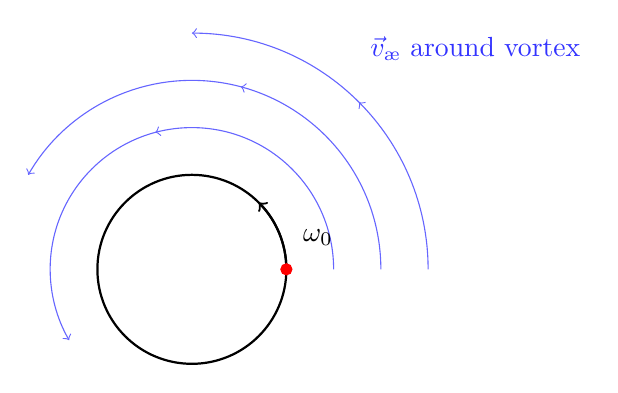
\begin{tikzpicture}[scale=2]
        \usetikzlibrary{decorations.markings}

        % Streamlines with varying arc lengths
        \draw[blue!60, ->,
            postaction={decorate},
            decoration={markings,
            mark=at position 0.5 with {\arrow{>}}}
        ] (0.9,0) arc (0:210:0.9); % Short arc

        \draw[blue!60, ->,
            postaction={decorate},
            decoration={markings,
            mark=at position 0.5 with {\arrow{>}}}
        ] (1.2,0) arc (0:150:1.2); % Medium arc

        \draw[blue!60, ->,
            postaction={decorate},
            decoration={markings,
            mark=at position 0.5 with {\arrow{>}}}
        ] (1.5,0) arc (0:90:1.5); % Long arc

        % Vortexring
        \draw[thick] (0,0) circle (0.6);
        \draw[thick, ->] (0:0.6) arc (0:45:0.6);
        \node at (0.8,0.2) {$\omega_0$};
        \filldraw[red] (0.6,0) circle (1pt);

        % Vectorveld label
        \node[blue!80] at (1.8,1.4) {$\vec{v}_{\ae}$ around vortex};

    \end{tikzpicture}
    \caption{Each $2\pi$ rotation of the vortex core = one tick of the internal clock.}
    \label{fig:wervelklok}
\end{figure}

In this model, a \grqq clock\textquotedblright is realized by a microscopic vortex's rotation. To make this concrete, consider a free particle at rest in the æther. Its vortex core spins steadily, dragging nearby æther around. Let $\omega_0$ denote the angular velocity of this core as measured in the æther rest frame (in units of radians per second). By definition, $\omega_0$ is the particle's \emph{proper rotational frequency}, corresponding to its proper time $\tau$.

We can relate $\omega_0$ to the passage of proper time: if the core rotates by $\Delta \theta$ radians in an interval, then the proper time elapsed is
\[
\Delta \tau = \frac{\Delta \theta}{\omega_0} \,.
\]
For example, if we choose $2\pi$ radians of rotation as a \("\)tick\("\) of the clock, then the proper period is $T_0 = 2\pi/\omega_0$. One might imagine $\omega_0$ is set by the particle's internal structure – e.g., a proton's vortex might rotate at some $10^{23}$ rad/s such that $T_0 \sim 10^{-23}$ s for one revolution (this is speculative, but notably, de Broglie in 1924 proposed that every particle of rest mass $m$ has an internal clock of frequency $mc^2/h$~\cite{deBroglie1924-frequency}, on the order of $10^{21}$ Hz for an electron; a vortex model could provide a physical origin for this \emph{Zitterbewegung} frequency as core rotation).

For now, $\omega_0$ is a free parameter representing the clock rate at rest. When the particle is not free or not at rest, its observed rotation rate can change. We define $\omega_{\textrm obs}$ as the angular velocity of the vortex core as observed by a static æther frame observer (i.e., one at rest with respect to the æther) under whatever circumstances (motion or gravity). The ratio $\omega_{\textrm obs}/\omega_0$ will then give the rate of the clock relative to proper time.

In fact, since $\Delta \tau = \Delta \theta / \omega_0$ always holds for the clock itself, and $\Delta t$ (coordinate time) corresponds to $\Delta \theta / \omega_{\textrm obs}$ (the angle rotated in lab frame time), we have:
\begin{equation}
\frac{\Delta \tau}{\Delta t} = \frac{\Delta \theta / \omega_0}{\Delta \theta / \omega_{\textrm obs}} = \frac{\omega_{\textrm obs}}{\omega_0} \,.
\end{equation}

This important relation links the physical slowdown of the vortex's spin $\omega_{\textrm obs}$ to the time-dilation factor. If $\omega_{\textrm obs} < \omega_0$, the clock runs slow (since $\Delta \tau < \Delta t$).

Our task in the next sections is to determine $\omega_{\textrm obs}$ for two cases:
\begin{enumerate}
    \item When the vortex (particle) moves at velocity $v$ through the æther,
    \item When the vortex sits in a gravitational potential (æther flow) created by a massive body.
\end{enumerate}
We will find that $\omega_{\textrm obs}/\omega_0$ in these cases reproduces the familiar Lorentz and gravitational time dilation factors, respectively.

Before we proceed, we emphasize that \emph{proper time $\tau$ in this model is fundamentally just a count of the rotation of the vortex}. This provides an objective, mechanistic picture of time: for example, one could imagine a small flag or marker on the vortex core completing laps around the core—each lap is an unambiguous physical event corresponding to a fixed amount of proper time. Different physical clocks (atoms, molecules, etc.) would all eventually trace their time to such microscopic circulations in the universal æther.

For a discussion of how composite clocks consisting of multiple vortex nodes collectively experience time dilation, see Appendix~ \hyperref[appendix:ClocksInVortexStructures]{A}

As long as the laws of physics are such that these circulations are stable and identical for identical particles, this provides a standard of time. We then show how motion through the æther and æther currents affect $\omega_{\textrm obs}$.